\chapter{Forforstærker}

Forforstærkeren har til opgave at forstærke mikrofonens udgangssignal til et liniesignals niveau. Et liniesignal har en amplitude fra 200 mV til 2 V og mikrofonens udgangssignal ligger, ifølge standarderne, mellem 0.8 mV og 200 mV \fixme{Den er jeg ikke helt sikker på}. 
Kravene fra kravspecifikationen som har indflydelse for designet af forforstærkerne er vist i tabel \ref{tab:krav_forforstaerker}.

\begin{table}[h]
\centering
\begin{tabular}{l|r|l}
\hline\hline
Område & Krav & Baggrund for krav \\
\hline\hline
Total Harmonic Distortion & \color{red}{<1 \%} & Ref til THD afsnit \\
Indgange & Linie og mikrofon & Se afsnit \ref{standarder} \\
Indgangsvælger & 3 trin & Se afsnit \ref{krav_indgangsvaelger} \\
Udgangssignaltype & Mono & Se afsnit \ref{krav_udgangssignaltype} \\
\textbf{Frontpanel:} & & \\
Indgangsvælger & Ja & Se afsnit \ref{krav_indgangsvaelger} \\
\textbf{Fjernbetjening:} & & \\
Indgangsvælger & Ja &  Se afsnit \ref{krav_fjernbetjening}\\
\hline\hline
\end{tabular}
\caption{Krav fra kravspecifikationen som har indflydelse på forforstærkeren}
\label{tab:krav_forforstaerker}
\end{table}



\section{Design}
Mikrofon kan maksimalt levere en outputspænding på 18 mV. Forforstærkeren skal forstærke dette til linjeniveau hvormed forstærkningen bliver: $2/18*10^(-3)=111$. Derfor er der valgt at benytte to CE med uafkoblet Re trin: ét der forstærker 10 gange og ét der forstærker 11 gange. Dette er vist på figur \ref{blok_forforstaerker}.

\begin{figure}[h]
\centering
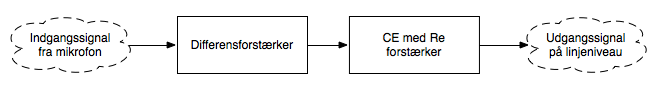
\includegraphics[scale=.6]{implementering/forforstaerker/blok_forforstaerker.png}
\caption{Blokdiagram over forforstærkerens byggeblokke samt lydsignalets vej}
\label{blok_forforstaerker}
\end{figure}

Udregningerne kan ses i vedlagt pdf (beregning_forforstaerker.pdf). 


\section{Simulering}


\section{Accepttest}

